\documentclass[preprint]{sigplanconf-eurosys}
\usepackage{graphicx}
\usepackage{arydshln}

\title{Global Namespaces Scale as Well as Decoupled Namespaces}
\authorinfo{Paper ID: 165}
           {Total Pages: 12}
\date{}
\begin{document}
\maketitle

% I work with the file system layer that sits on top of Ceph
% - internal subsystems and interfaces that Ceph uses to provide a strongly consistent POSIX file system
%   - e.g., load balancing mechanisms, for hotspots/flash crowds on directories
%     caches for inodes, capabilities for guarding a shared resource, and a large journal for fault tolerance
% - our programmability initiative talks about composing these internal interfaces for higher level services

% 
% Previous work: 
% - master's thesis: scale-out vs. scale-up architectures 
% - work in industry: file systems for the cloud, big data processing over
% object storage, and automating workflows
%
% I work under Carlos at UC Santa Cruz and we study how to migrate file system
% metadata to alleviate overloaded servers. The idea is to take the namespace
% on one metadata server, chop it up into smaller subtrees, and farm those
% subtrees out to other metadata servers.  It's very similar to IndexFS/ShardFS
% but we try to leverage namespace locality by allowing variable sized
% subtrees. We published a paper at SC'15 where we talk about a load balancing
% API we built on CephFS that let's administrators control how to chop up
% subtrees and when/where to move them (also got merged into Ceph).
%
% Go to conclusion
%
% Why I want to work with Brad
% - new perspectives on file system designs, especially NON-POSIXy 
% - work in a national lab: I know about theirarchitectures and problems but
% I've never used an HPC system - real world applications and benchmarks; most
% of my work has been accepted for novelty but not for fully benchmarking a
% system
% - lines up with my thesis
%
% What I want to work on:
% - continue working on my thesis; this next phase of having a global namespace
% but different consistency semantics within that namespace for data management
%   - namespace: recursive data structure as a logical model for understanding the user's goals
%   - merge: what is the proper way to merge deltafs/batchfs updates back into the global namespace
%   - data management: deltaFS made the case that apps shouldn't use the fs to synchronize;
%     we contend that you could use the fs as data management; remembering how to access your data
%
% What I have been working on 
% - leverage internal services/subsystems in Ceph; avoids code duplication and
% let's us test this over the same system 
% - benchmarking the overheads of strong consistency/journalling - we've figured
% out how to thrash capabilities and turn off the journal
\begin{abstract}

Today's large and highly-parallel workloads are bottlenecked by metadata
services because many processes end up accessing the same shared resoure. In
HPC, state-of-the-art file systems are abandoning POSIX because the
sychronization and serializiation overheads are too costly -- and sometimes
even unnceccessary -- for some of their applications.  While the performance
benefits are plain for these users, other applications that rely on stronger
consistency must be re-written or deployed on a different system.  We present
Cudele, a programmable file system that supports different degrees of
consistency and fault tolerance within the same namespace.  First, we take a
POSIX compliant file system and relax the consistency constraints by
implementing two metadata designs: delayed metadata update merge into the
global namespace and client local views of metadata updates.  Second, we store
the consistency and fault tolerance semantics in inodes so that subtrees within
the same namespace can be optimized for different workloads; the inodes are
programmable so that clients understand how to access the metadata in a
subtree.  Third, we present a theoretical framework for a metadata service and
a working implementation that provides the lowest common denominator needed to
implement a wide range of consistency/fault tolerance semantics that can be
benchmarked all on the same system.

\end{abstract}

% Questions
% - do you still collaborate with CMU? Would you want all of us to work together?
% - what projects do you want to work on?
% - how closely would you want to work with Carlos?
% - what system would you want to work on?

% The main difference between CephFS and the CMU systems is that our approach
% is a little more flexible.  We can partition the namespace in any way and can
% co-locate items together if they are dependent on each other -- in theroy...
% in practice it is very hard to figure out what the workload is trying to do.
% Also, we can program the decision making based on different metrics, like
% CPU, request rate, etc.

\section{Introduction}

Today's client-server based file system metadata services have scalability
problems. It takes a lot of resources to server POSIX metadata requests and
applications perform better with dedicated metadata
servers~\cite{sevilla:sc15-mantle, ren:sc2014-indexfs}. This is fine for small
workloads and file systems but as the system scales provisioning a metadata
server for every client is expensive and complicated.

Current hardware evolution and the rise of software-defined storage storage,
which uses techniqes like erasure coding, replication, and partitioning, have
ushered a new era of HPC computing; architectures are transitioning from
complex storage stacks with burst buffer, file system, object store, and tape
tiers to a two layer stack with just a burst buffer and object
store~\cite{bent:login16-hpc-trends}. This trend exacerbates the metadata
scalability problem and has given rise to the serverless metadata services.

HPC workloads are so metadata intensive that new management techniques are
advocating reducing synchronization and serialization overheads by transferring
these responsibilities to the client. We call this approach decoupling the
namespace and the semantics of consistency differ amongst systems.

\begin{figure}[tb]
\centering
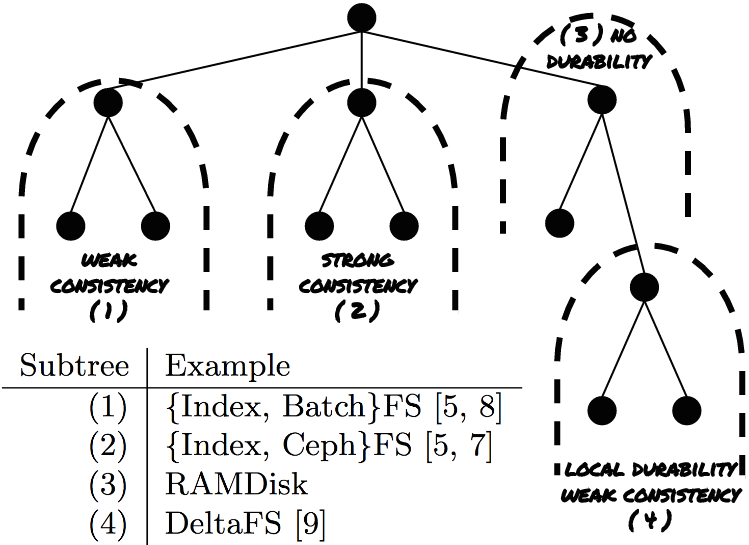
\includegraphics[width=75mm]{figures/subtree-policies.png}
\caption{Administrators can assign consistency and fault tolerance policies to
subtrees to get the benefits of some of the state-of-the-art HPC architectures.
}\label{fig:subtree-policies}
\end{figure}

We propose subtree policies, an interface that lets future programmers control
how the system manages different parts of the namespace.  For performance one
subtree can adopt weaker consistency semantics while another subtree can retain
the rigidity of POSIX's strong consistency. Figure~\ref{fig:subtree-policies}
shows an example setup where a single global namespace has directories for
applications designed for different, state-of-the-art HPC architectures.  Our
system supports 3 forms of consistency and 2 forms of fault tolerance giving
the administrator a wide range of policies and optimizations depending on the
application's needs.

\section{Related Work} 

% General
The bottlenecks associated with accessing POSIX file system metadata are not limited
to HPC workloads and the same challenges that plagued these systems for years are
finding their way into the cloud. Workloads that deal with many small files
({\it e.g.}, log processing and database
queries~\cite{thusoo:sigmod2010-facebook-infrastructure}) and large numbers of
simultaneous clients ({\it e.g.}, MapReduce
jobs~\cite{mckusick:acm2010-gfs-evolution}), are subject to the scalability of
the metadata service. The biggest challenge is that whenever a file
is touched the client must access the file's metadata and maintaining a file
system namespace imposes small, frequent accesses on the underlying storage
system~\cite{roselli:atec2000-FS-workloads}.  Unfortunately, scaling file
system metadata is a well-known problem and solutions for scaling data IO do
not work for metadata IO~\cite{roselli:atec2000-FS-workloads,
abad:techreport2012-fstrace, abad:ucc2012-mimesis,
alam:pdsw2011-metadata-scaling, weil:osdi2006-ceph}. There are two approaches
for improving the performance of metadata access.

\subsection{Metadata Load Balancing}

% approaches to load balancing (strong = more resuorces per unit work, weak =
% fixed resource per work unit)
One approach for improving metadata performance and scalability is to alleviate
overloaded servers by load balancing metadata IO across a cluster. Common
techniques include partitioning metadata when there are many writes and
replicating metadata when there are many reads. For example, IndexFS partitions
directories and clients write to different partitions by grabbing leases and
caching ancestor metadata for path traversal; it does well for strong scaling
because servers can keep more inodes in the cache which results in less RPCs.
Alternatively, ShardFS replicates directory state so servers do not need to
contact peers for path traversal; it does well for read workloads because all
file operations only require 1 RPC and for weak scaling because requests will
never incurr extra RPCs due to a full cache.  CephFS employs both techniques to
a lesser extent; directories can be replicated or sharded but the caching and
replication policies do not change depending on the balancing technique.
Despite the performance benefits these techniques add complexity and jeopardize
the robustness and performance characteristics of the metadata service because
the systems now need (1) policies to guide the migration decisions and (2)
mechanisms to address inconsistent states across servers.

% policies
Setting policies for migrations is arguably more difficult than adding the
migration mechanisms themselves.  For example, IndexFS and CephFS use the
GIGA+~\cite{GIGA+} technique for partitioning directories at a predefined
threshold and using lazy synchronization to redirect queries to the server that
``owns" the targeted metadata.  Determining when to partition directories and
when to migrate the directory fragments are policies that vary between systems:
GIGA+ partitions directories when the size reaches a certain number of files
and migrates directory fragments immediately; CephFS partitions directories
when they reach a threshold size or when the write temperature reaches a
certain value and migrates directory fragments when the hosting server has more
load than the other servers in the metadata cluster. Another policy is when and
how to replicate directory state; ShardFS replicates immediately and
pessimistically while CephFS replicates only when the read temperature reaches
a threshold.  There is a wide range of policies and it is difficult to address
with tunables and hard-coded design decisions.

% addressing inconsistency
In addition to the policies, distributing metadata across a cluster requiress
distributed transactions and cache coherence protocols to ensure strong
consistency ({e.g.}, POSIX).  For example, ShardFS pessimistically replicates
directory state and uses optimistic concurrency control for conflicts; namely
it does the operation and if there is a conflict at verification time it falls
back to two-phase locking.  Another example is IndexFS's inode cache which
reduces RPCs by caching ancestor paths -- the locality of this cache can be
thrashed by random reads but performs well for metadata writes. For
consistency, writes to directories in IndexFS block until the lease expires
while writes to direcotries in ShardFS are slow for everyone as it either
requires serialization or locking with many servers; reads in IndexFS are
subject to cache locality while reads in ShardFS always resolve to 1 RPC.
Another example of the overheads of addressing inconsistency is how CephFS
maintains client sessions and inode caches for capabilities (which in turn make
metadata access faster). When metadata is exchanged between metadata servers
these sessions/caches must be flushed and new statistics exchanged with a
scatter-gather process; this halts updates on the directories and blocks until
the authoratitive metadata server responds.  These protocols are discusssed in
more detail in the next section but their inclusion here is a testament to the
complexity of migrating metadata.

%For metadata writes it does a distributed transaction; monotonic writes with
%concurrent clients fail and do pessimistic locking through a mediated lock
%server to ensure strong consistency, non-monotonic writes grab locks at every
%server. Zooming in on monotonic writes: if permissions increase it executes on
%a primary then non-primary, if permissions decrease it executes on all
%non-primary then on primary.

The conclusion we have drawn from this related work is that metadata protocols
have a bigger impact on performance and scalability than load balancing.  
Understanding these protocols helps load balancing and gives us a better
understanding of the metrics we should use to make migration decisions ({\it
e.g.}, which operations reflect the state of the system), what types of
requests cause the most load, and how an overloaded system reacts ({\it e.g.},
increasing latencies, lower throughput, etc.).

\subsection{Relaxing POSIX}

% POSIX 
POSIX workloads require strong consistency and many file systems improve
performance by reducing the number of remote calls per operation ({\it i.e.}
RPC amplification). As discussed in the previous section, caching with leases and
replication are popular approaches to reducing the overheads of path traversals
but their performance is subject to cache locality and the amount of available
resources, respectively; for random workloads larger than the cache extra RPCs
hurt performance~\cite{IndexFS, CephFS} and for write heavy workloads with more
resources the RPCs for invalidations are harmful. Another approach to reducing
RPCs is to use leases or capabilities.  


%IndexFS aggressively caches paths and
%handles permissions by handing out leases for metadata writes; metadata may
%only be modified when all leases have expired. 
%IndexFS~\cite{ren:sc2014-indexfs} aggressively caches pathnames and their
%permissions on the client servers. Modifications to metadata cached by clients
%is delayed until all client leases have expired. This reduces the RPC
%amplification to 1 when mutatating directory metadata ({\it e.g.,}
%\texttt{mkdir}, \texttt{chmod}, etc.) because clients are not querying MDSs for
%path traversals. The disadvantage of this approach is the high latency of
%mutation operations (reads to filenames).  ShardFS~\cite{xiao:socc2015-shardfs}
%replicates metadata (specifically directory lookup state) across the MDS
%cluster, reducing the RPC amplification to 1 for file operations ({e.g.,}
%\texttt{stat}, \texttt{chmod}, \texttt{chown}, etc.). Modifications to the
%directory lookup state are done with optimistic concurrecny control and fall
%back to retry if verification fails. The disadvantage of this appraoch is the
%high number of RPCs for maintaining directory metadata mutations (writes to
%directories).  CephFS also maintains an inode cache but its notion of leases
%are much shorter, on the order of microseconds.

% Non POSIX
High performance computing has unique requirements for file systems ({e.g.},
fast creates) and well-defined workloads (e.g., workflows) that make relaxing
POSIX sensible.  One popular approach is to allow clients to ``lock'' parts of
the namespace to improve performance and scalability by avoiding
synchronization, false sharing, and serialization.  BatchFS assumes the
application coordinates accesses to the namespace, so the clients can batch
local operations and merge with a global namespace image lazily. Similarily,
DeltaFS eliminates RPC traffic using subtree snapshots for non-conflicting
workloads and middleware for conflicting workloads. MarFS gives administrators
the ability to (1) lock ``project directories" and (2) allocate GPFS clusters
for demanding directory workloads. TwoTiers eliminates high-latencies by
storing metadata in a flash tier; apps lock the namespace so that metadata can
be accessed more quickly.  Unfortunately, decoupling the namespaces has costs:
(1) merging metadata state back into the global namespace is slow; (2) failures
are local to the failing node; and (3) the systems are not backwards
compatible. 

% NON POSIX
%Decoupling the namespaces has many advantages, including improved scalability,
%higher resource utilization, and better performance.  BatchFS and DeltaFS are
%near-POSIX filesystems that give clients the ability to decouple subtrees from
%the namespace so that the applications can execute metadata operations without
%synchronization and serialization.  These operations are applied to a local
%snapshot of the file system namespace and conflicts are resolved either by the
%application or by an external service . Applications link into a metadata
%server library to reduce resource utilization and code paths (e.g., no daemons
%and less interprocess communication). 

For (1), state-of-the-art systems manage consistency in non-traditional ways:
IndexFS maintains the global namespace but blocks operations from other clients
until the first client drops the lease, BatchFS does operations on a snapshot
of the namespace and merges batches of operations into the global namespace,
and DeltaFS never merges back into the global namespace. The merging for
BatchFS is done by an auxiliary metadata server running on the client and
conflicts are resolved by the application. Although DeltaFS never explicitly
merges, applications needing some degree of ground truth can either manage
consistency thesmelves on a read or add a bolt-on service to manage the
consistency.

For (2), if the client fails and stays down, all metadata operations on the
decoupled namespace are lost. If the client recovers, the on-disk structures
(for BatchFS and DeltaFS this is the SSTables used in TableFS) can be
recovered. In other words, the clients have state that cannot be recovered if
the node stays failed and any progress will be lost. This scenario is a
disaster for checkpoint-restart where missed cycles may cause the checkpoint to
bleed over into computation time.

For (3), decoupled namespace approaches sacrifice POSIX going as far as
requiring the application to link against the systems they want to talk to. In
today's world of software defined caching, this can be a problem for large data
centers with many types and tiers of storage. Despite well-known performance
problems POSIX and REST are the dominant APIs for data transfer.

Decoupling the namespace delays metadata consistency and sacrifices fault
tolerance. As shown in Table~\ref{table:namespaces}, metadata consistency is
provided by capabilities and fault tolerance is addressed with a journal.

\begin{tabular}{ r | l | l | l }
              & Decoupled & Global    & Implied   \\
              & Namespace & Namespace & Namespace \\\hline
  Example     & BatchFS & CephFS & PLFS \\
              & DeltaFS & IndexFS &     \\
  Consistency & eventual & strong & none? \\
  Fault Tol.  & node local & journal & journal \\
\end{tabular}

\section{POSIX Overheads}

\begin{figure}[tb]
\centering
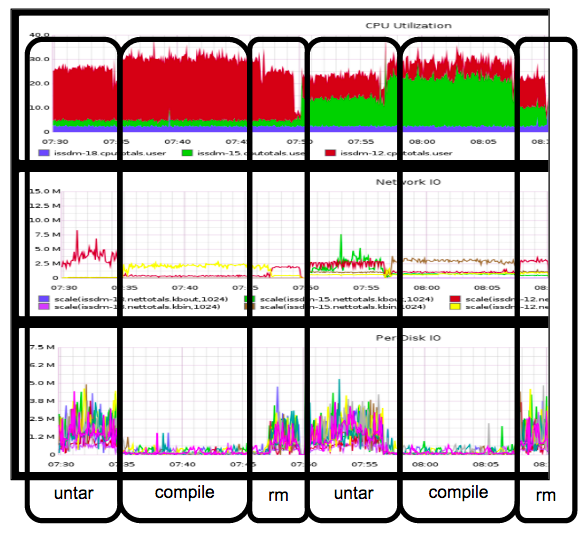
\includegraphics[width=75mm]{figures/creates-motivation.png}
\caption{Create-heavy workloads (untar) incurr the highest disk, network, and CPU
utilization because the metadata server is managing consistency and fault
tolerance.}\label{fig:creates-motivation}
\end{figure}

In our examiniation of the overheads of POSIX we benchmark and analyze CephFS,
the file system that uses the RADOS object store to store its data and
metadata. We choose CephFS because it is an open-source production quality
system. CephFS made one set of design decisions and we not asserting that the
design decisions that were made are superior but instead highlight the
effect those decisions have on performance.

To show how CephFS behaves under high metadata load we use a create-heavy
workload because these types of workloads incurr high CPU, network, and disk
usage.  Figure~\ref{fig:creates-motivation} shows a compilation of the Linux
kernel, which has a download, untar, compile, and remove phase. The untar phase
is characterized by many creates and has the highest resource usage, indicating
that it is stressing the consistency and journalling subsystems of the metadata
server. Also of note: a create-heavy workload does not help for caching indoes.

In this section, we quantify the costs of consistency and fault tolerance in
CephFS. If the components that ensure these semantics (i.e. capabilities and
journals, respectively) can be mitigated or delayed, then global namespaces
perform as well as decoupled namespaces. We run our experiments on a 9 OSD, 3
MDS, 1 MON Ceph cluster. The clients use the Ceph kernel client, which has been
in the mainline Linux kernel since TODO. We use the kernel client so that we
can find the true create speed of the server; our experiments show a low CPU
utilziation for the clients which indicates that we are stressing the servers
more. We also turn caching off becuase, as shown in figureX there is little
difference, in terms of performance between caching and not caching when using
the kernel client.

\subsection{Fault Tolerance}
\label{sec:fault-tolerance}
\begin{figure*}[tb] \centering
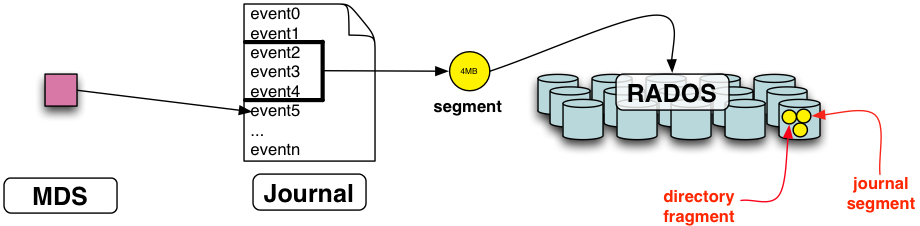
\includegraphics[width=1\textwidth]{./figures/journal.png} 
\caption{CephFS uses a journal to stage updates and tracks dirty metadata in
the collective memory of the MDSs. Each MDS maintains its own journal, which is
broken up into 4MB segments. These segments are pushed into RADOS and deleted
when that particular segment is trimmed from the end of the log. In addition to
journal segments, RADOS also stores per-directory objects. \label{fig:journal}}
\end{figure*}

\begin{figure*}[tb]%h
\centering
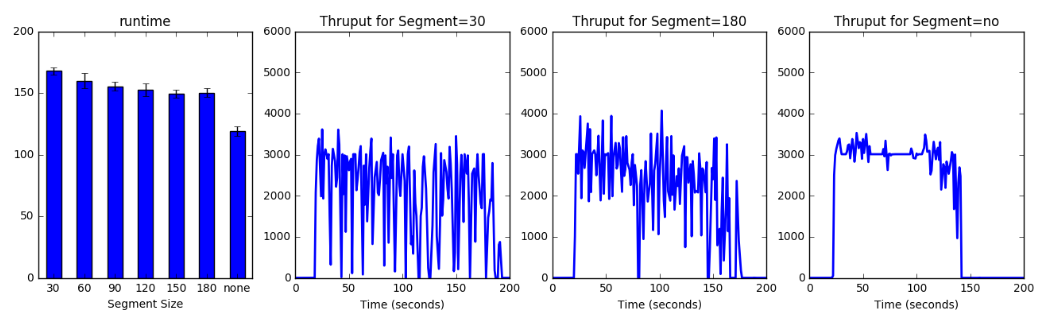
\includegraphics[width=180mm]{figures/throughput-journal.png}
\caption{Performance improves with larger journal segments because the metadata
server spends less time flushing the journal }\label{fig:throughput-journal}
\end{figure*}

%\begin{figure}[tb]%h
%\centering
%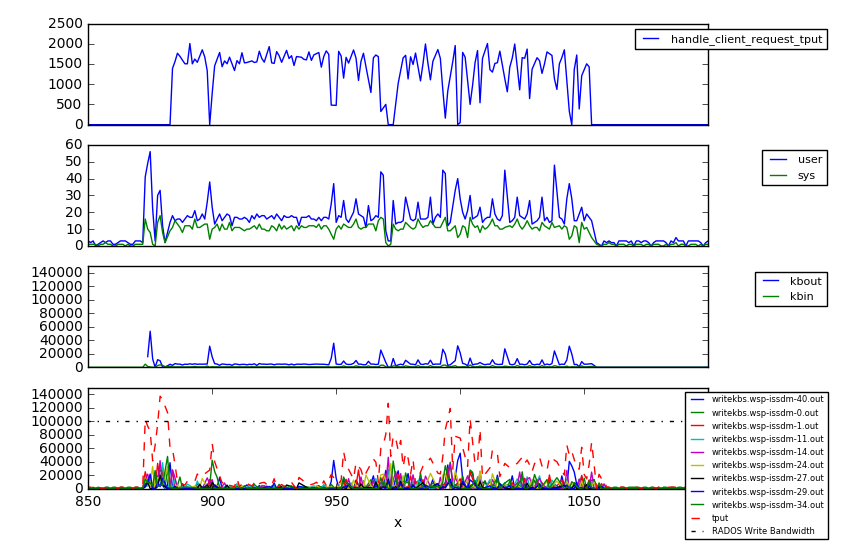
\includegraphics[width=80mm]{figures/throughput-journal-old.png}
%\caption{(a), (b), and (c) show increased activity halfway though the run; (d)
%shows that this activity is related to disk IO, indicating that the activity is
%the journal.  Despite the activity, we conclude that RADOS itself is not the
%bottleneck because our RADOS cluster can sustain 100MB/s write bandwidth.
%}\label{fig:throughput-journal-old}
%\end{figure}
%Figure~\ref{fig:throughput-cache} shows that journaling metadata updates into
%the object store has an overhead.  (a) shows that throughput degrades halfway
%through the run; (b) shows that cpu utilization spikes at this same point; (c)
%shows that outgoing network utilization spikes; and (d) shows that this
%activity spikes on the disks in RADOS.

% purpose of the journal
As shown in Figure~\ref{fig:journal} CephFS uses RADOS (1) as a metadata store
for all information about files including the hierarchical namespace and (2) as
a staging area for the journal of updates before they are applied to the
metadata store. (1) is essentially a cache that improves performance by serving
metadata from memory and (2) is the mechanisms for achieving fault tolerance. 

% - sequential IO, trim redundant operations
Fault tolerance means that the client or server can fail and metadata will not
be lost.  CephFS addresses fault tolerance with a metadata journal that streams
into the resilient object store. Similar to LFS~\cite{} and WAFL~\cite{} the
metadata journal can grow to large sizes ensuring (1) sequential writes into
RADOS and (2) the ability for daemons to trim redundant or irrelevent journal
entries. 

% Knobs in CephFS
The journal is striped over objects where multiple journal updates can reside
on the same object. There are two tunables for controlling the journal: the
segment size and the number of parallel segments that can be written in
parallel. The former is memory bound as larger segments take up more memory but
can reduce the time spent journaling and the latter is CPU bound. 

% Effects on performance
Figure~\ref{fig:throughput-journal} shows that journaling metadata updates into
the object store has an overhead. Part (a) shows the runtime for different
journal segment sizes; the larger the segment size the bigger that the writes
into the object store are. The trade-off comes is in terms of memory because
larger segment sizes take up more space with their buffers. Parts (b), (c), and
(d) show the throughput over time for different segment sizes. Performance
suffers when time is spent journaling. 

% Conclusion
Despite this overhead, we posit that the journal is sufficient to slow down
metadata throughput but not so much as to overwhelm RADOS because we measured
our peak bandwidth to be 100MB/s, which is the speed of our network link.

\textbf{Comparison to decoupled namespaces}: In BatchFS and DeltaFS, as far as
we can tell, when a client or server fails there is no recovery scheme. For
BatchFS, if a client fails when it is writing to the local log-structured
merged tree (implemented as an SSTable) then those batched metadata operations
on lost. For DeltaFS, if the client fails then on restart the computation does
the work again -- since the snapshots of the namespace are never globally
consistent, there is no ground truth the requires the failed namespace to
answer to anyone. On the server side, BatchFS and DeltaFS use IndexFS. Again,
IndexFS writes metadata to SSTables but it is not clear whether they ever
vacate memory, get written to disk, or are flushed to the object store.

\subsection{Strong Consistency} 

\begin{figure*}[tb]%h
\centering
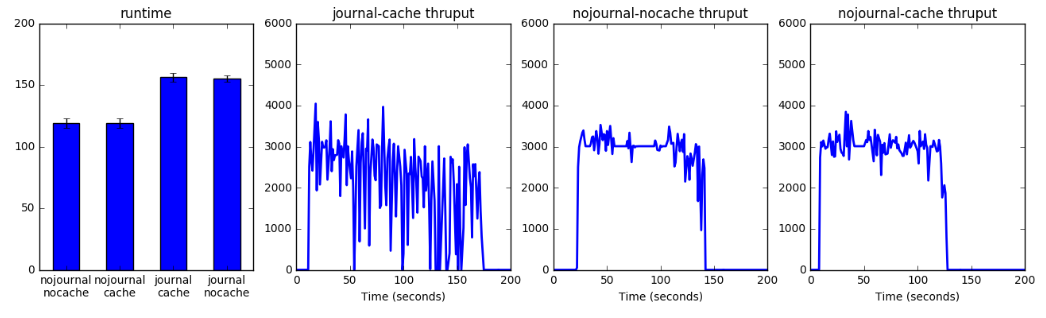
\includegraphics[width=180mm]{figures/throughput-cache-journal.png}
\caption{Journalling metadata updates has a bigger overhead than maintaining
the inode cache. For create-heavy workloads the inode cache offers no
performance benefits. }\label{fig:throughput-cache-journal}
\end{figure*}

\begin{figure*}[tb]%h
\centering
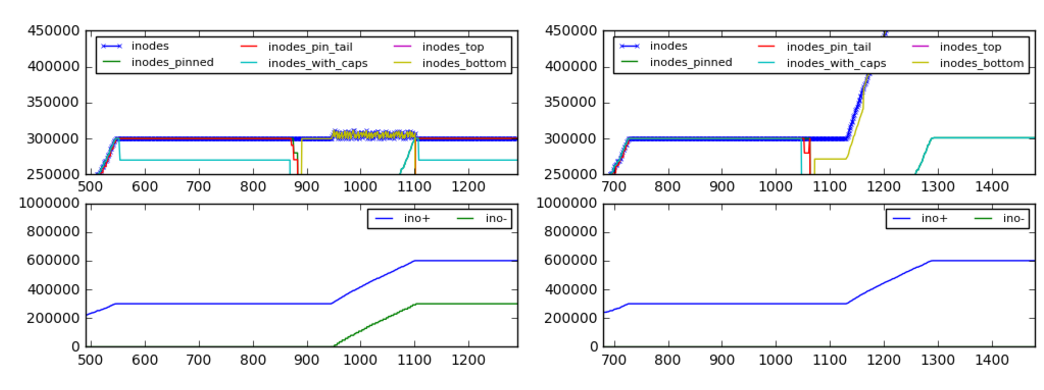
\includegraphics[width=180mm]{figures/inode-cache.png}
\caption{The inode cache improves metadata read performance but for our
create-heavy workload it is only an overhead. Most of the time maintaining the
cache is spent evicting and adding inodes.}\label{fig:inode-cache}
\end{figure*}

Access to POSIX metadata is strongly consistent, so reads and writes are
globally ordered. The synchronization and serialization machinery needed to
ensure that all clients see the same state has high overhead.  CephFS uses
capabilities to keep metadata strongly consistent. To reduce the number of RPCs
needed for consistency, clients can obtain capabilities for reading, reading
and updating, reads caching, writing, buffering writes, changing the file size,
and performing lazy IO.

\begin{figure*}[tb]%h
\centering
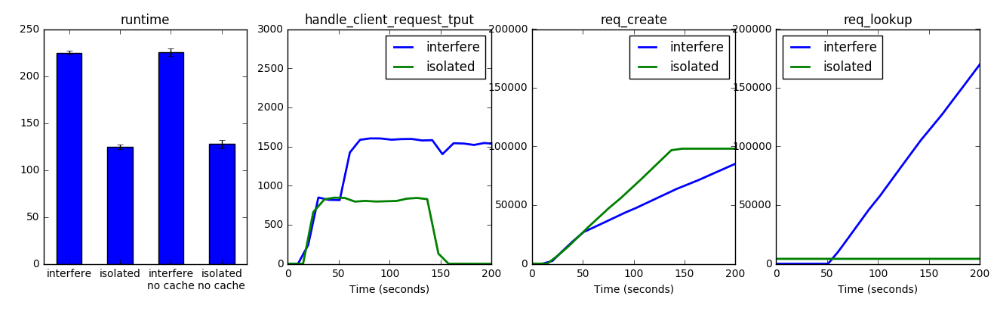
\includegraphics[width=180mm]{figures/throughput-droplease.png}
\caption{When a client create stream is ``isolated" then lookups resolve
locally but when a second client ``interferes" by creating in the same directory,
the directory inode capability is revoked forcing all clients to centralize
lookups at the metadata server.  \label{fig:throughput-droplease}}
\end{figure*}

% purpose of the inode ccahe - reduces RPCs (lookups for create, readdirs for
% stats)
To keep track of the read caching and write buffering capabilities, the clients
and metadata servers agree on the state of each inode using an inode cache.  If
a client has the directory inode cached it can do metadata writes (e.g.,
create) with a single RPC. If the client is not caching the directory inode
then it must do multiple RPCs to the metadata server to (1) determine if the
file exists and (2) do the actual create.  Unless the client immediately reads
all the inodes in the cache, the inode cache is less useful for create-heavy
workloads because the cached inodes are unused. 

% benefits
The benefits of caching the directory inode when creating files is shown in
Figure~\ref{fig:throughput-droplease}(a).  If only one client is creating files
in a directory (``isolated" curve) then that client can lookup the existence of
new files locally before issuing a create request to the metadata server. If
another client starts creating files in the same directory (``interfere" curve)
then the directory inode transitions out of read caching and the first client
must send lookups to the metadata server. When other clients interfere the
request throughput is higher Figure~\ref{fig:throughput-droplease}(b) but the
runtime is slower because the isolated client scenario incurrs less requests.
Figures~\ref{fig:throughput-droplease}(c) and (d) plot the creates and lookups,
repsectively, over time; creates slow down and lookups dominate the request
load when the directory inode is shared in the interferring client scenario.

% TODO: what is the cost of trimming the cache?
% TODO: does CephFS still cache inodes when I turn off caching? Why is still keeping inodes in memory? Gah!
%\begin{figure}[tb]%h
%\centering
%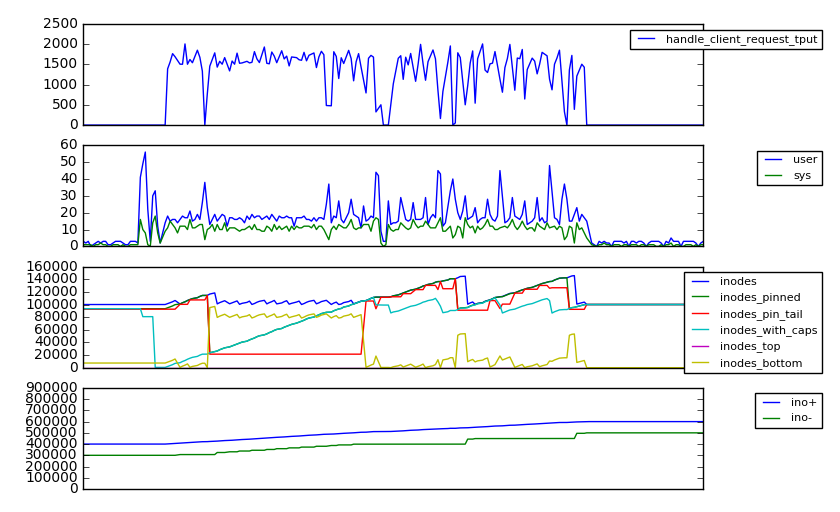
\includegraphics[width=80mm]{figures/throughput-cache.png}
%\caption{ CephFS tries to maintain 100 thousand inodes in the cache;
%performance degrades when it cannot evict inodes fast enough to maintain this
%threshold. \label{fig:throughput-cache}}
%\end{figure}

% disadvantages
The drawbacks of the inode cache are shown in
Figure~\ref{fig:throughput-cache}.  Figure~\ref{fig:throughput-cache}(a) shows
the throughput in metadata requests per second for a single client creating 200
thousand files. Until time 950 the throughput is steady at just under 2000
ops/sec and the CPU utilization is at about 30\%. At time 950 seconds
throughput degrades which corresponds to more inodes in the cache
(Figure~\ref{fig:throughput-cache}(c)). The values in
Figure~\ref{fig:throughput-cache}(c) are:

\begin{itemize}
  \item inodes: total number of elemnts in the cache
  \item inodes pinned: 
  \item inodes pinned tail
  \item inodes with caps
  \item inodes top
  \item inodes bottom 
\end{itemize}

% how the inode cache works
CephFS tries to keep the cache at 100 thousand inodes so the degradation in
performance indicates that the metadata server cannot keep up with the
workload. Figure~\ref{fig:throughput-cache}(d) shows inodes getting added at
the same rate as before 950 seconds (ino\(+\)) but the rate at which inodes get
removed is less stable (ino\(-\)) indicating that cache eviction is taking more
of the metadata servers time.

\subsection{Consistency Overhead}
\begin{figure*}[tb]
\centering
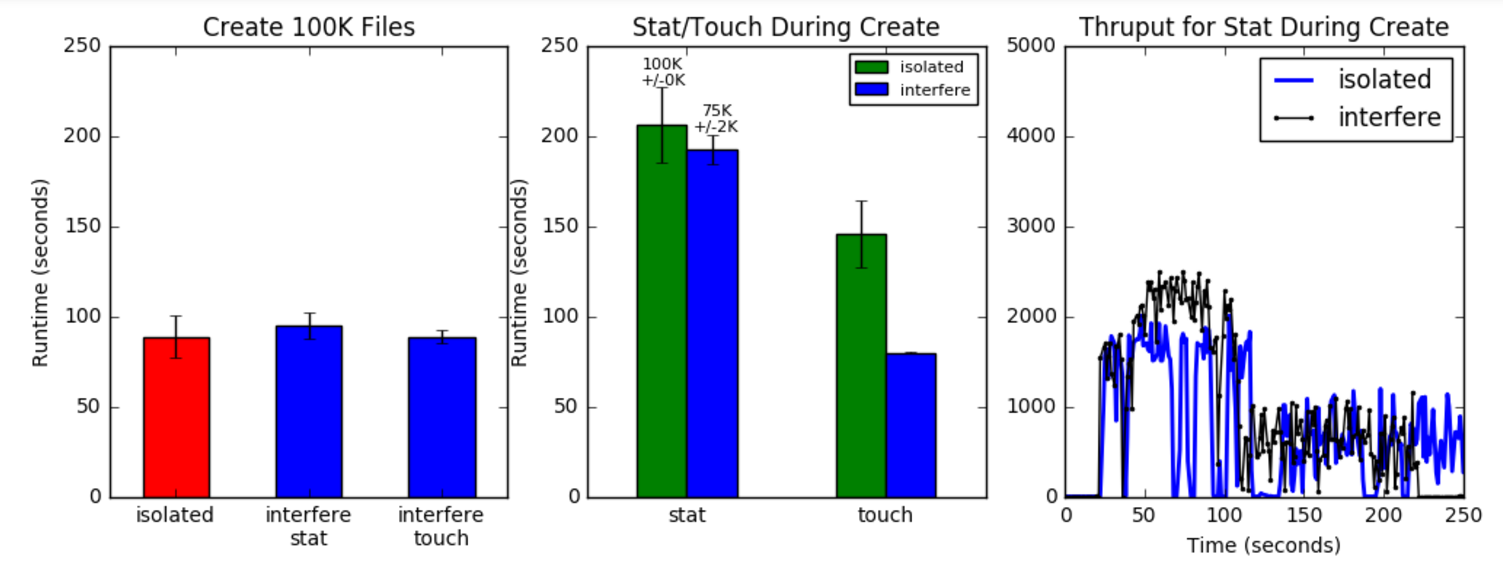
\includegraphics[width=180mm]{figures/exp0-underloaded.png}
\caption{An underloaded metadata server adaquately services conflicting
clients; the create speeds are similar while the interferring operations are
limited by the cost of RPCs.}\label{fig:exp0-underloaded}
\end{figure*}

\begin{figure*}[tb]
\centering
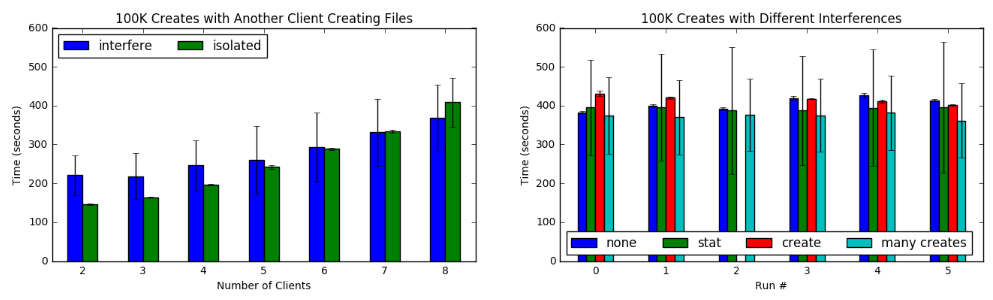
\includegraphics[width=180mm]{figures/runtime-consistency-scale.png}
\caption{Scaling clients shows increased variability when another client
interferes; zooming in on runs with 7 clients we see that different types of
interferring operations have different effects on performance variability and
predictability.  }\label{fig:runtime-consistency-scale}
\end{figure*}

Figure~\ref{fig:exp0-underloaded} is a baseline showing that the metadata
server can service multiple clients when it is underloaded. One client creates
files in the same directory and another does a touch or stat 15 seconds into
the run. Figure~\ref{fig:exp0-underloaded}(a) shows the runtime of the client
doing the creates: "isolated" is when the create client is the only workload in
the cluster, "interfere stat" is the runtime of the create client when another
client does a stat, and "interfere touch" is the runtime of the create client
when another client does a touch. There is only a minor performance
degradation. Figure~\ref{fig:exp0-underloaded}(b) compares the baseline
the other client doing the touch or stat
%
%and Figure~\ref{fig:exp0-underloaded}
%has a throughput trace to show behavior.
%
%In Figure~\ref{fig:exp0-underloaded}(a), 
%creates only see a minor performance
%degradation while the interferring operations in
%Figure~\ref{fig:exp0-underloaded}(b) show a larger (yet not significant)
%discrepency. 
%
%
%
% isolated is when there is no interferrence from client 1.
To explain Figure~\ref{fig:exp0-underloaded}(a) we use
Figure~\ref{fig:exp0-behaviour}(b) to show why the runtime of creating 100
thousand files is unaffected. Compared to the throughput without an
interferring stat ("isolated" curve) the throughput of the metadata server with
an interferring stat ("inteferring stat" curve) is higher. This means the
metadata server is doing more operations suggesting that it can adequately
handle the demands of both workloads.  

To explain Figure~\ref{fig:exp0-underloaded}(b) we use
Figure~\ref{fig:exp0-underloaded}(a) to show that operations are bounded by the
number of files; more files incurr more requests since both operations lookup
every file. The number of files shown in Figure~\ref{fig:exp0-behaviour}(a)
indicates that the local stat ("client 0" bar) is interacting with less files
than the remote stat ("client 1" bar). This graph also explains why the
isolated stats and touches take the longest from the remote clients; out of all
setups, the isolated operations are doing the most RPCs.  The difference
between local ("client 0 interfere" bar) and remote ("client 1 interfere" bar)
in Figure~\ref{fig:exp0-underloaded}(b) is the overhead of doing RPCs.
Isolated is the slowest because it requests the most files. On average the
local interferring client ("client 0" bar in
Figure~\ref{fig:exp0-behaviour}(a)) requests 40 thousand less files than the
remote interferring call ("client 1" bar in
Figure~\ref{fig:exp0-behaviour}(a)). This reflects how fast the local client
can get into the queue of requests, presumably because it bypasses capability
checks.

From this experiment we make 2 conclusions: (1) the metadata server is not
overloaded because it can handle both workloads and (2) the metadata server
needs to get global consistency from only 1 client

\textbf{Comparison to decoupled namespaces}: Decoupled namespaces merge batches
of metadata operations into the global namespaces when the job completes.  In
BatchFS the merge is delayed by the application using an API to switch between
asynchronous to sychronous mode. The merge itself is explicitly managed by the
application but future work looks at more automated methdologies. In DeltaFS
snapshots of the metadata subtrees stays on the client machines; there is no
ground truth and consistent namespaces are constructed and resolved at
application read time or when a 3rd party system (e.g., middleware, scheduler,
etc.) needs a view of the metadata.

\section{Methodology: Decoupled Namespaces}

\begin{figure}[tb]
\caption{Applications can decouple the namespace, write updates to a local
journal, and delay metadata updates.  Table~\ref{table:spectrum} shows how
these phases (represented by the arrows) can be combined to provide weaker
consistency or fault tolerance semantics.  }\label{fig:decouple}
\centering
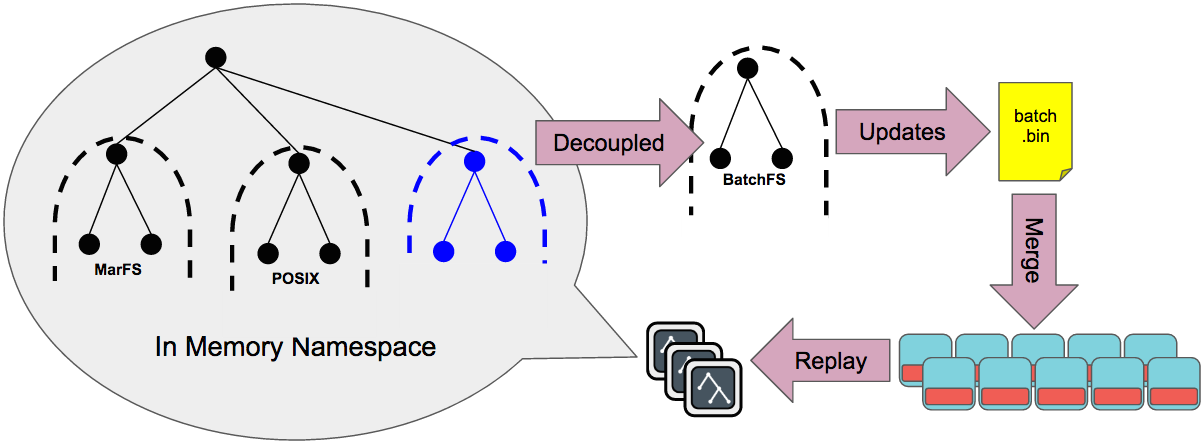
\includegraphics[width=90mm]{figures/fig-decouple.png}
\end{figure}

In this section we describe Cudele, our prototype system that lets future
programmers compose mechanisms (Section~\S\ref{sec:cudeles-mechanisms}) to
provide the necessary guarantees
(Section~\S\ref{sec:setting-policies-with-cudele}) for their application.

\subsection{Cudele's Mechanisms}
\label{sec:cudeles-mechanisms}

% describe the figure
Figure~\ref{fig:decouple} shows the mechanisms (labeled arrows) in Cudele and
which entity they are performed by (gray boxes). The metadata store and journal
are different ways of representing the namespace. The metadata store represents
the namespace as a tree of directory fragments and is easier to read/traverse.
On the other hand, the journal represent the namespace as a list of events. It
a ``pile system"; writes are fast but reads are slow because state must be
reconstructed.  Specifically, reads are slow because there is more data to
read, it is unorganized, and many of the updates may be redundant.

% describe the mechanisms
Cudele presents 6 mechanisms: RPCs, Stream, Create, Volatile Apply, Save, and
Persist. ``RPCs" does round trip remote procedure calls to establish
consistency; it is the default implementation for complying with POSIX in
CephFS. ``Stream" has the metadata servers stream a journal of metadata updates
into the object store. ``Create" allows clients to append metadata events to an
in-memory journal. ``Volatile apply" takes the in-memory journal on the client
and applies it directly to the in-memory metadata store of the metadata server
cluster. ``Save" takes the in-memory journal and writes it to the client's
disk. ``Persist" saves the journal as a an object in the object store from the
client.

Next, we discuss how these mechanisms can be composed to get different
consistency and fault tolerance semantics. 

%\begin{tabular}{ r | l }
%  \(\Rightarrow\)   & Description \\\hline
%  create            & events appended to in-memory journal \\
%  v.apply           & journal volatily applied to in-memory metadata store \\
%  save              & journal saved to client's disk \\
%  persist           & journal saved in object store \\
%  replay            & metadata servers materialize namespace \\
%  RPCs              & round trip remote procedure calls \\
%  stream            & metadata server streams journal into RADOS \\
%\end{tabular}

\subsection{Setting Policies with Cudele}
\label{sec:setting-policies-with-cudele}

\begin{table}[t]
\begin{center}
\caption{Cudele lets future programmers explore the spectrum of consistency and
fault tolerance semantics shown below.\label{table:spectrum}}
\begin{tabular}{ r | l | l | l }
  consistency     \(\rightarrow\) &&& \\  
  fault tolerance \(\downarrow\)  & none & eventual & global \\\hline
  none   & create   & create   & RPCs    \\
         &          & +v.apply &         \\\hdashline
  local  & create   & create   & RPCs    \\
         & +save    & +save    & +save   \\
         &          & +v.apply &         \\\hdashline
  global & create   & create   & RPCs    \\
         & +persist & +persist & +stream \\
         &          & +v.apply &         \\
\end{tabular}
\end{center}
\end{table}

% describe table
The spectrum of consistency and fault tolerance guarantees that adminstrators
can construct is shown in Table~\ref{table:spectrum}. The columns are the
different consistency semantics and the rows cover the spectrum of fault
tolerance guantees. For consistency: ``none" means the system does not handle
merging updates into a global namespace and it is assumed that middleware or
the application manages consistency lazily; ``eventual" merges updates either
when the system has time (e.g., by a background daemon) or when the client is
done writing; and updates in ``global" consistency are seen immediately by all
clients. For fault tolerance, ``none" means that updates are volatile and will
be lost on a crash of any component. Stronger guarantees are made with
``local", which means updates will be retained if the client node recovers, and
``global", where all updates are always recoverable.

% which system they represent and which are impossible
The cells in Table~\ref{table:spectrum} encompass many exisiting storage
systems. POSIX systems like CephFS and IndexFS have global consistency and
fault tolerance; DeltaFS has consistency and fault tolerance set to ``none";
and BatchFS uses ``eventual" consistency and ``local" fault tolerance. These
are just a few of the HPC examples.  

% how its done
To compose the mechanisms administrators inject which steps (described in
Section~\S\ref{sec:cudeles-mechanisms}) to run and which to use in parallel
using a domain specific language. For example, to get the semantics of BatchFS,
the administrator would inject the following pipeline:\\

\noindent \texttt{create+save+v.apply}\\

% what is impossible
Although we can achieve all permutations of the different guarantees in
Table~\ref{table:spectrum}, not all of them make much sense. For example, it
makes little sense to do \texttt{creates+RPCs} since both steps do the same
thing or \texttt{stream+save} since global fault tolerance is stronger and has
more overhead than local fault tolerance.  Formulaically, valid steps
include:\\

\noindent \texttt{<create|RPCs> [+v.apply][+save][+persist][+stream]}

\subsection{Subtree Policies}

\section{Implementation}
\label{sec:implementation}

% Outline of the section
Each section below corresponds ot the labeled arrows in
Figure~\ref{fig:decouple}. This implementation decouples policies from
mechanisms allowing applciations to choose the consistency and fault tolerance
semantics they need.

% Programmability
Of the 6 mechanisms in Figure~\ref{fig:decouple} 4 had to implemented and only
1 required changes to the underlying storage system itself.  RPCs and stream
can be achieved with tunables in configuration files for the storage system
(e.g., metadata cache size, logging on/off, etc.).  Persist", save, and create
are implemented as library and does not require modifications to the storage
system. Volatile apply requires changes to the metadata server to inject
updates back into the global namespace. 

\subsection{No Changes: RPCs, Stream}

RPCs is the default behavior of the storage system. Depending on the cache
state and configuration each operation incurrs at least RPC. For example, if a
client or metadata server is not caching the directory inode, all creates
within that directory will result in a lookup and a create request. If the
directory inode is cached then only the create needs to be sent.

Re-using the debugging and testing features in the storage system, we can turn
stream on and off. If it is off, then the metadata servers will not save
journals in the object store and the daemons that apply the journal to the
metadata store will never run. Performance numbers for enabling and disabling
the stream phase are presented back in Section~\S\ref{sec:fault-tolerance}.

% General information about the journal
The journal segments are saved as objects in RADOS.  The journal has 4
pointers, described in `osdc/Journaler.h`:

\begin{itemize}
  \item write position: tail of the journal; points to the current session where we are appending events
  \item unused field: where someone is reading
  \item expire position: old journal segments
  \item trimmed position: where daemon is expiring old items
\end{itemize}

% How the journal tool works
Journal segments in RADDS have a header followed by serialized log events. The
log events are read by hopping over objects using the read offset and object
size pulled from the journal header.  After decoding them, we can examine the
metadata (1) about the event (e.g., type, timestamps, etc.) and (2) for inodes
that the event touches.

% The metablobs
The metadata for inodes that the event touches are called metadata blobs and
the ones associated with events are \textbf{unordered}; this layout makes
writing journal updates fast but the cost is realized when reading the metadata
blobs.  It makes sense to optimize for writing since reading only occurs on
failures. To reconstruct the namespace for the metadata blob, the journal tool
iterates over each metadata blob in the events and builds mappings of inodes to
directory entries (for directories) and parent inodes to child inodes/directory
entries.

\subsection{External Library: Create, Save, Persist}
%Reads/Writes Journal Events}

% How it works
For ``create", ``save", and ``persist" Cudele provides a library for clients to
link into.  Recall that CephFS uses the object store (1) as a metadata store
for all information about files including the hierarchical namespace and (2) as
a staging area for the journal of updates before they are applied to the
metadata store. As discussed previously, the metadata store is optimized for
reading while the journal is optimized for writing.  Cudele re-uses the journal
tool to read/write log events to memory and persistent storage.

% creates
The journal tool is used for disaster recovery and lets administrators view and
modify the journal of metadata updates; it can read the journal, erase events
from the journal, and apply the updates in the journal to the metadata store.
To apply journal updates to the metadata store, the journal tool reads the
journal segments from object store objects and applies the update to the
metadata store (which are also stored as object store objects).  For create,
clients write to an in-memory journal and updates are merged into the global
namespace by replaying them onto the metadata store in the object store.  

% Journal import
The journal tool imports journals from binary files stored on disk.  First the
header of the dump is sanity checked and written into RADOS to the ``header"
object.  The ``header" object has metadata about the journal as well as the
locations of all the journal pointers (e.g., where the tail of the journal is,
where we are currently trimming, etc.).  Then the journal events are cleaned
(erasing trailing events that are not part of the header) and written as
objects into RADOS.  Note that while the journal is in RADOS, the metadata
servers do do not have the namespace reconstructed in memory so the metadata
cluster will not service requests relating to the journal of imported events.
To construct the namespace in the collective memory of the metadata servers we
need to first construct the namespace in RADOS. The journal tool can explicitly
do this by  applying the journal to the metadata store in RAODS. This will pull
the objects containing journal segments and replay them on the metadata store.
Finally, we delete the journal in RADOS and restart the metadata servers so
they rebuild their caches.

% Journal export
The journal tool exports journals to binary files stored on disk. First the
journal is scanned for the header and then journal is recovered. To recover the
journal the ``header" object is read off disk and then objects are probed in
order and starting from the write position saved in the header. Probing will
update the write position if it finds objects with data in them. 

% Journal export
When exporting a journal of events, the journal tool first scans the journal to
check for corruption. Then it recovers the journal by reading the ``header"
object out of RADOS.  After reading the header, the journal tool can pull
journal segments from RADOS because it knows how many objects to pull and how
far to seek within those objects.

%% The data structures
%The metadata that the event touches, including inodes, paths, and timestamps,
%are stored as metablobs. Each piece of metadata inside a metablob is called a
%dirlump. A dump has a section for lumps (dirfrag, dirlump), roots (dentries),
%table client transactions (tid, version), renamed directory fragments (maps,
%versions, alloc/preallocated inodes), inodes starting a truncate, inodes
%finishing a truncate, destroyed inodes, and client requests. Unfortunately for
%me (and you since you are reading this paper), this does not make any sense.
%
%Each directory fragment has an associated directory lump, which is just a bunch
%of metadata. The most interesting part of the dirlump is the fullbits array,
%which has a dentry OR inode. To walk the tree, iterate over all the dirlumps
%and then all the full bits, saving off the children and inode locations. The
%children tell us which dentry names an inode has and the inode locations map
%the parent inode to its child inode and dentry.  

% persist/save
For save, clients write serialized log events to a file on local disk and for
persist, clients store the file in the objects store. The overheads for save
and persist is the write bandwidth of the local disk and object store,
respectively.

% Level of intrusion
This required no changes to Ceph because the metadata server knows how to read
the events we were writing into the object store.  The client writes metadata
updates locally and merges the updates with the journal tool. The client that
decouples the namespace operates without any consistency and any conflicts at
the merge are resolved in favor of this client. Updates by other clients ({\it
i.e.} metadata writes to the global namespace) are overwritten.  We leverage
the journal tool's ability to reconstruct metadata events in memory. The client
library is shown in Figure~\ref{fig:decouple}.  Cudele adopts the following
process when an application decouples the namespace:

\begin{enumerate}
  \item ``\textbf{decoupled}": metadata server exports the journal events to a file
  \item ``\textbf{transfer}": the file is pulled by the client from the metadata server
  \item ``\textbf{snapshot}": client reads the file and materializes a snapshot of the
        namespace in memory
\end{enumerate}

% Why we re-use stuff
By using re-using the journal subsystem to implement the namespace decoupling,
Cudele leverages the write/read optimized data structures, the formats for
persisting events (similar to TableFS's SSTables), and the functions for
replaying events onto the internal namespace data structures.  

%Step 3 is the most complicated and requires understanding how the snapshot is
%materialized in memory. 
%
%\subsubsection{Operating on Snapshots} 
%
%Our first implementation attempted to re-create journal events using the same
%libraries that the metadata server uses. To construct a \texttt{mkdir} we tried
%to instantiate a Ceph inode and directory entry for the current file/dir and
%its parent.  This is too hard because there are too many moving parts in the
%metadata server (e.g., a mdlog class, stuff in memory, assumption that we can
%traverse up and down namespace, etc.). So when I tried add dentries and inodes
%it was trying to traverse up/down and it would almost always segfault when it
%was looking for something. These metablobs are supposed to be self container --
%the problem is I do not know what is supposed to go *inside* them. 
%
%Our second idea was to copy the metadata blog and change just what we needed.
%For example, we would save a binary dump of a generic \texttt{mkdir} event on
%disk. When the application makes a directory, this dump would be loaded and the
%fields would be changed before being written back to disk. Rather than
%traversing up and down a namespace in memory of a metadata server, we should
%traverse up and down the namespace *inside* the metadata blob. This
%implementation requires disk IO and editing the log event is non-trivial for
%two reasons:
%
%\begin{itemize}
%
%  \item methods do not edit events; they just write them
%
%  \item the metadata that the event touches (e.g., the metablob) is unorganized
%  on disk for performance -- it is trade-off for writing data faster serially and
%  reconstructing information slowly since failure is not considered the norm
%
%\end{itemize}
%
%Faced with these challenges we landed on our final implementation: load the
%snapshot into the the data structures used to examine and replay journals, edit
%those data structures, and write them out to disk as binary.

\subsection{Storage System Changes: Volatile Merge}

%The metadata objects are located with naming schemes (200.000* for journal
%objects and 1.inode for metadata storage objects). 

% How it works: socket for changing daemon's internal state (debugging, logging, behaviour)
% 1. API for putting state into the daemon dynamically
% 2. Hooks directly into daemon code so we can use any parsing functionality in there
% 3. Documentation all the tunables

% 1. read journal of updates from file
% 2. call replay (uses same code as when an MDS comes back) on each event
% 3. skip inodes so MDS doesn't hand out those new inodes

\section{Results}
\subsection{Microbenchmarks}
\begin{figure*}[tb]
\centering
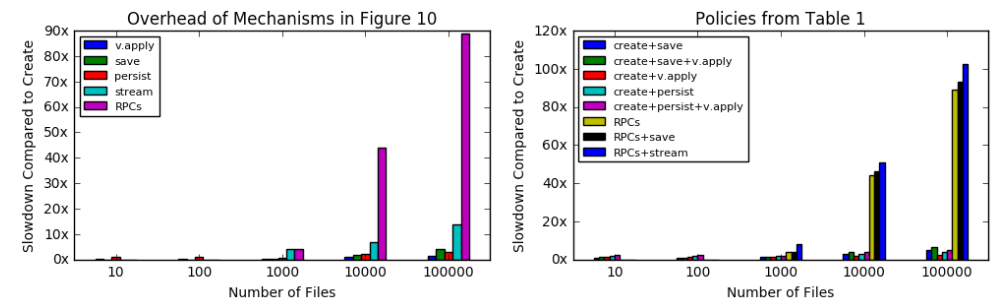
\includegraphics[width=180mm]{figures/results-microbenchmark.png}
\caption{Here's a graph.}
\end{figure*}

\begin{figure}[tb]
\centering
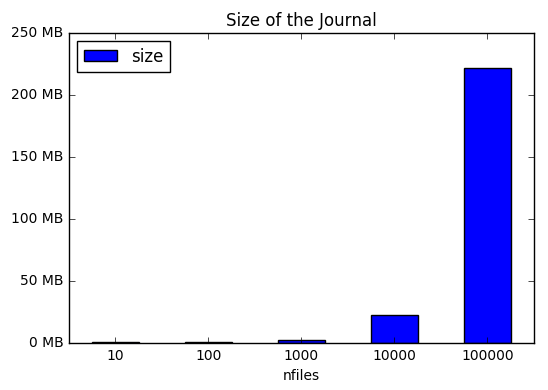
\includegraphics[width=90mm]{figures/results-files.png}
\caption{Here's a graph.}
\end{figure}


\subsubsection{Per phase latencies}
\begin{figure}[tb]
\centering
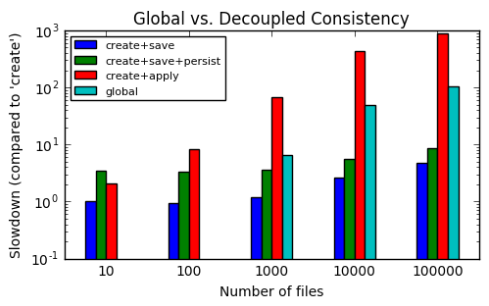
\includegraphics[width=90mm]{figures/global-v-decoupled.png}
\caption{Compared to the \texttt{create} phase, saving and persisting
updates (\texttt{create+save} and \texttt{create+save+persist}) experience only
a 4.79\(\times\) and 8.66\(\times\) slowdown, in the worst case for 100K files.
In contrast, maintaining \texttt{global} consistency is 905.70\(\times\)
slower.  The disadvantage of decoupling the namespace is the merge phase where
updates are applied to the metadata store (\texttt{create+apply}, resulting in a
905.70\(\times\) slowdown for 100K files.}\label{fig:global-v-decoupled}
\end{figure}

%\section{notes}
%Linking clients into our custom libcephfs
%
%Use namespace's recursive data structure to put policies on subtrees
%- consistency: eventual vs. strong, global vs. local
%  - e.g., BatchFS/DeltaFS: eventual, local
%  - e.g., POSIX: strong, global
%  - e.g., PLFS: no consistency
%- fault tolerance: global vs. local
%  - e.g., CephFS: global
%  - e.g., BatchFS/DeltaFS: local
%
%Experimental Setup
%- Ceph: 9 OSDs, 1 MDS, 2 kernel client
%- Workload limitations: blah
%
%Workload: creates
%
%Baseline: 200K creates in the same directory
%- throughput: degrades at 950s
%- CPU utilization: more at 950s
%- inode cache: eviction dominate
%- inodes +- to cache: eviction dominate
%- per-disk throughput: RADOS not bottleneck
%
%Experiment 1: Interference
%
%\subsection{Baseline}
%Experiment 0: creates in the same directory
%- setup: why we use caching, we use the kernel client, how we circumvent max fragment size
%
%Experiment 0: creates with a stat
%- Hypothesis: metadata read pauses creates and requires a snapshot in time
%  - what is more of an overhead: pausing creates and getting a consistent view OR sucking up resources as it reads from RADOS?
%- can we delay snapshot?
%
%Experiment 1: creates with a readdir
%- Hypothesis: shows the cost of synchronization because on a write, the first client drops his caps
%- client0: create 100k, client1: stat at 2 mins
%
%Experiment 2: scale the number of files
%- See if the open/close spike occurs 
%- Try to see why open/close spike is allowed to happen
%- Try to disable all caching -- metadata writes don't ever re-use the inode -- we never ask for it again!
%- client0: create 100k, client1: touch at 2 mins
%
%Experiment 3: see how fast the cache satisfies a read
%- client0: create 100k, stat inodes
%- client0: create 100k, client1: stat inodes
%
%lient 0: creates, client 1 create(s)

\subsection{Journaling Overhead}

Journal to RADOS
Turn off journaling (large segment)
Journal to in-memory OSD 

\subsection{Macrobenchmarks}
updatedb: http://lists.ceph.com/pipermail/ceph-users-ceph.com/2015-July/002768.html

\bibliography{paper}
\bibliographystyle{plain}
\end{document}
